% !TEX root = ./main.tex
% !TEX encoding = UTF-8 Unicode
% !TEX program = pdflatex
% !TeX spellcheck = it_IT

\chapter{Processing on Databricks}

\section{Drop dati}
In seguito è riportato il codice utilizzato per il drop di informazioni superflue
o ridondanti dai data frame a disposizione.
\begin{figure}[!htbp]
	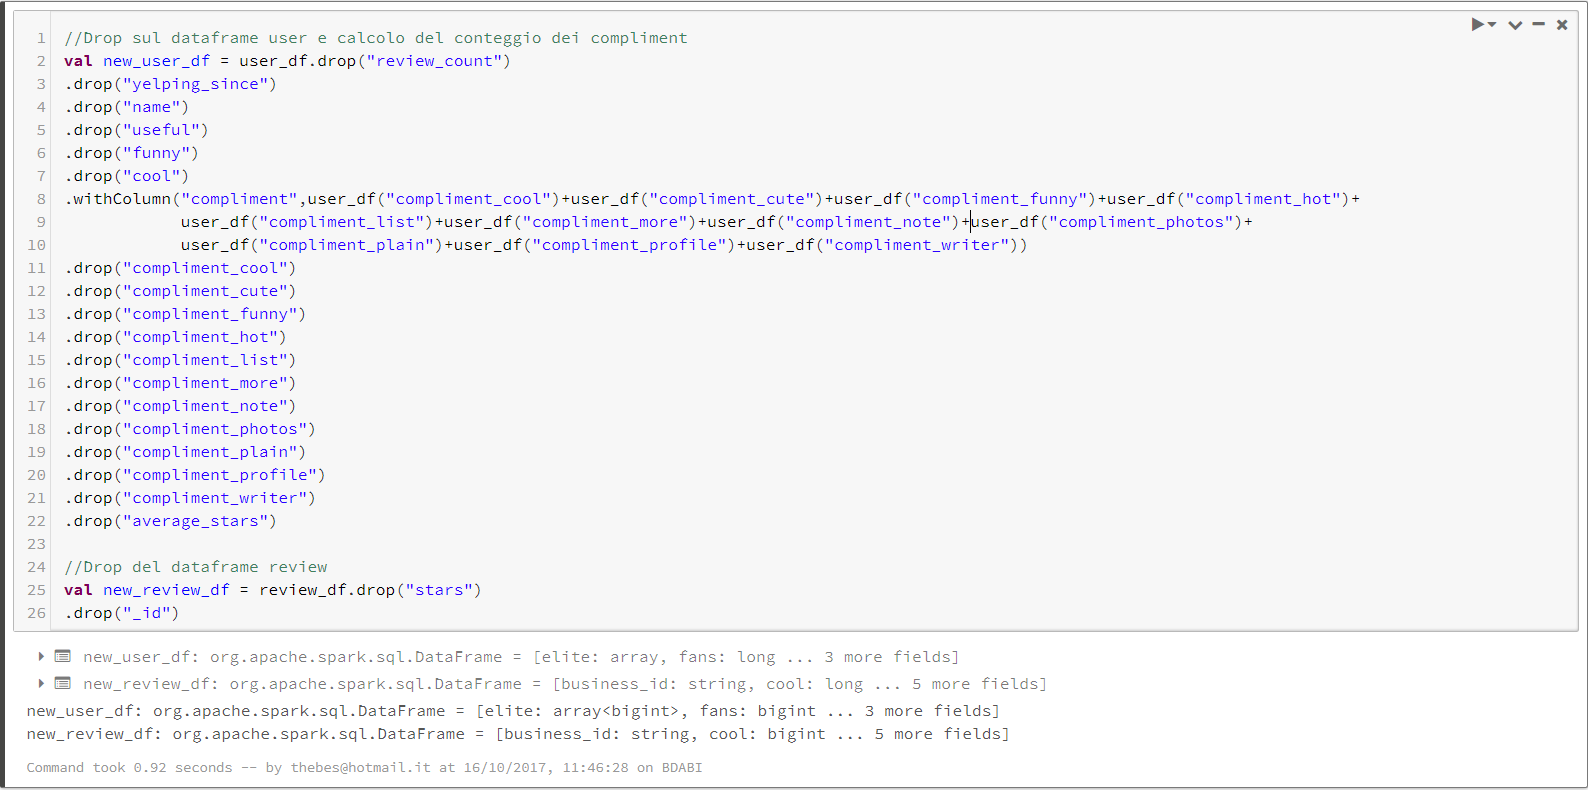
\includegraphics[width=1\linewidth,keepaspectratio]{command_1}
	\caption{Codice per il drop degli attributi superflui}
	\label{command_1}
\end{figure}

\clearpage

\section{Filtraggio Reviews}

\begin{figure}[!htbp]
	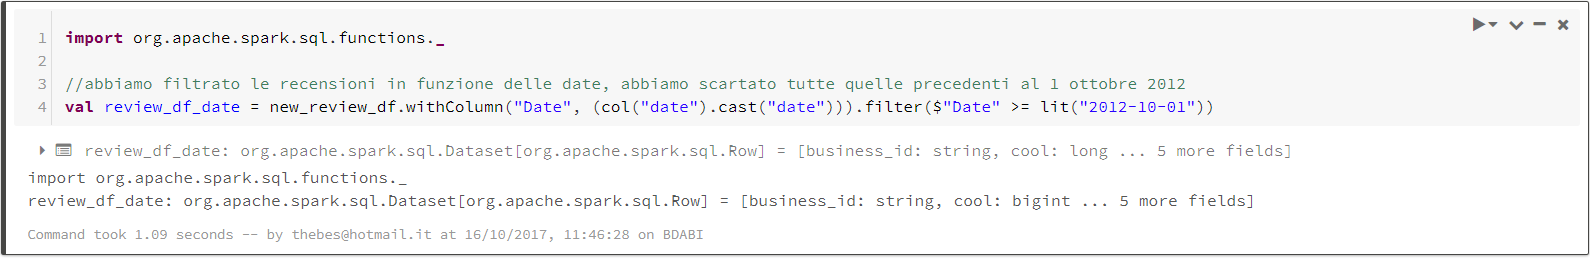
\includegraphics[width=1\linewidth,keepaspectratio]{command_2}
	\caption{Filtraggio delle reviews successive al 1 Ottobre 2012}
	\label{command_2}
\end{figure}

\clearpage

\section{Calcolo attributi di Scoring per Users}
\subsection{Creazione attributo \textit{Elite Score}}
La seguente command filtra gli utenti che hanno il titolo di ``\textit{Elite 2017}''
ed inoltre assegna loro un punteggio dato dalla somma degli anni in cui sono
stati eletti elite.
\begin{figure}[!htbp]
	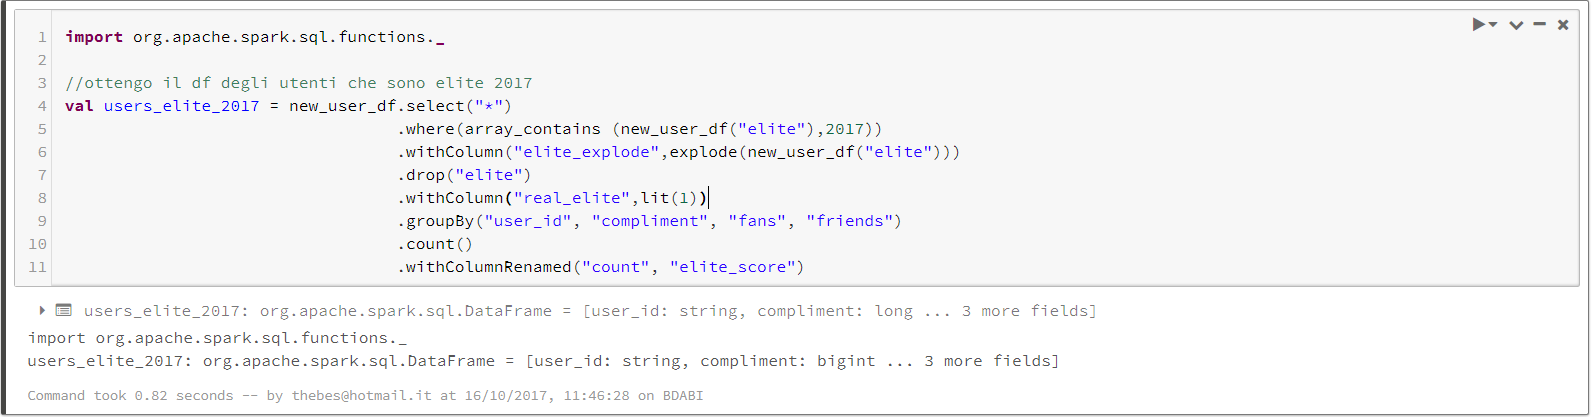
\includegraphics[width=1\linewidth,keepaspectratio]{command_3}
	\caption{Filtraggio degli utenti elite 2017}
	\label{command_3}
\end{figure}

La seguente command filtra gli utenti che non hanno il titolo di ``\textit{Elite 2017}''
ed inoltre assegna loro un punteggio nullo.
\begin{figure}[!htbp]
	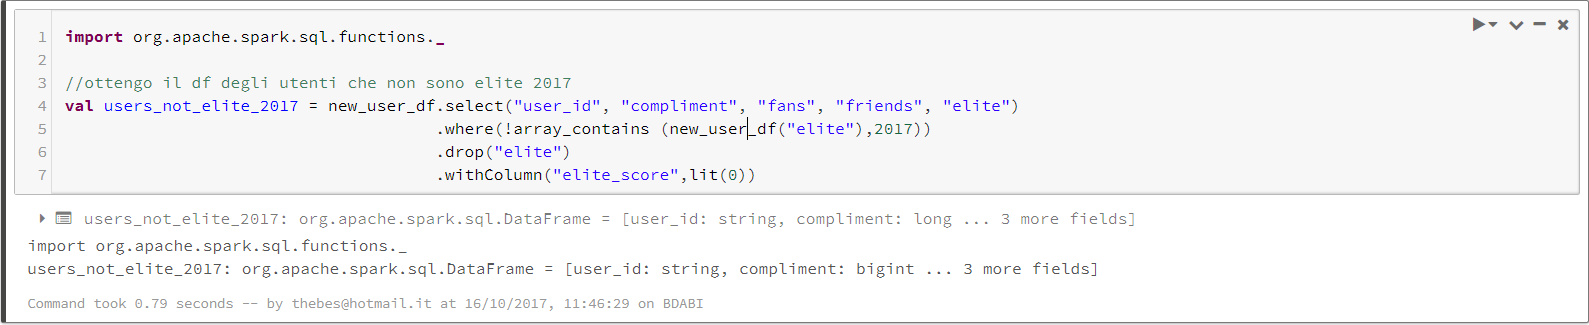
\includegraphics[width=1\linewidth,keepaspectratio]{command_4}
	\caption{Filtraggio degli utenti non elite 2017}
	\label{command_4}
\end{figure}

La seguente command crea un nuovo data frame Users, aggiungendo il nuovo campo
numerico \textit{elite}
\begin{figure}[!htbp]
	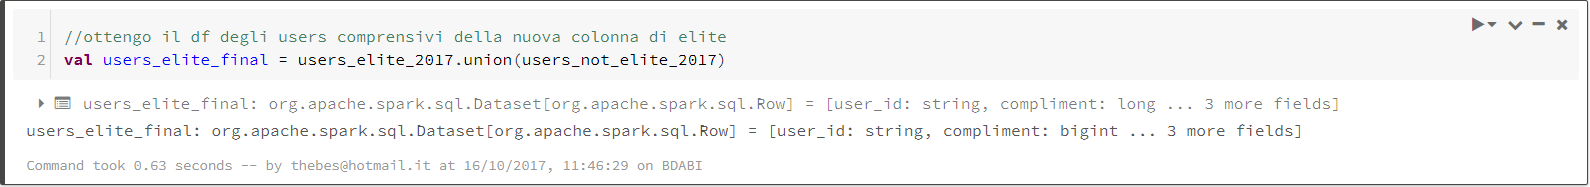
\includegraphics[width=1\linewidth,keepaspectratio]{command_5}
	\caption{Creazione data frame users contenente il nuovo campo \textit{elite}}
	\label{command_5}
\end{figure}

\subsection{Creazione attributo \textit{Reviews Score}}
La seguente command calcola la combinazione lineare pesata degli attributi \textit{funny},
\textit{cool}, e \textit{useful}.\\
I pesi sono stati assegnati al fine di dar maggiore importanza a quelli che
sono apparsi essere più significativi per l'analisi effetuata.
\begin{figure}[!htbp]
	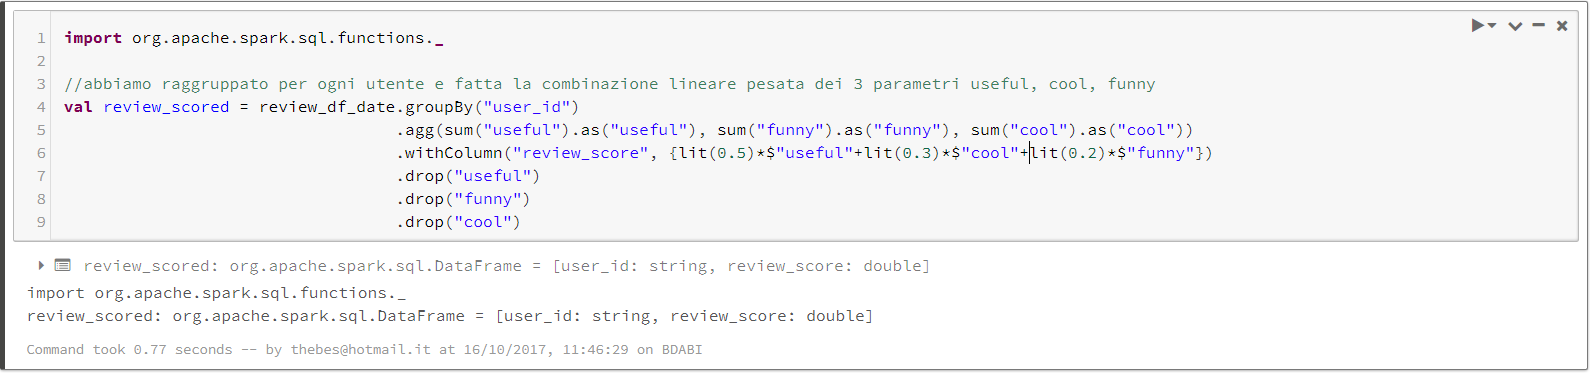
\includegraphics[width=1\linewidth,keepaspectratio]{command_6}
	\caption{Creazione attributo \textit{review\_score}}
	\label{command_6}
\end{figure}

La seguente command crea un nuovo data frame che comprende il valore review\_score
calcolato.
\begin{figure}[!htbp]
	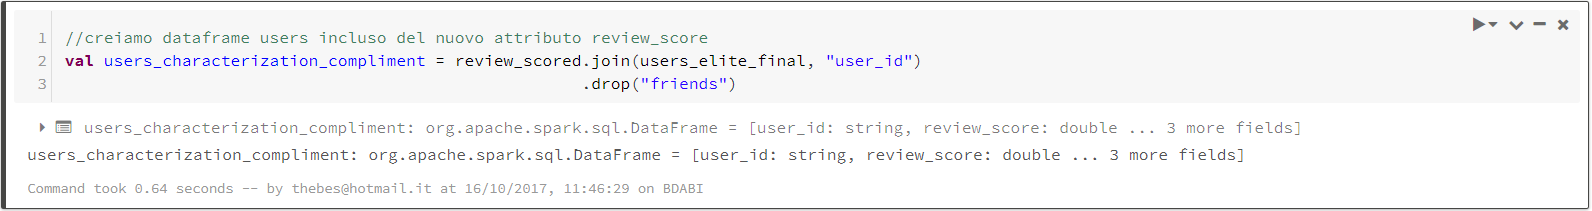
\includegraphics[width=1\linewidth,keepaspectratio]{command_7}
	\caption{Aggiunta \textit{review\_score} al data frame users}
	\label{command_7}
\end{figure}

\clearpage

\section{Creazione data frame degli edges(relazioni user-user) con peso archi}
La seguente command prepara un data frame iniziale user\_relations in cui ogni tupla
soddisfa la proprietà che \textbf{User2} ha recensito almeno \textit{dieci}
business già precedentemente recensiti da \textbf{User1}.
\begin{figure}[!htbp]
	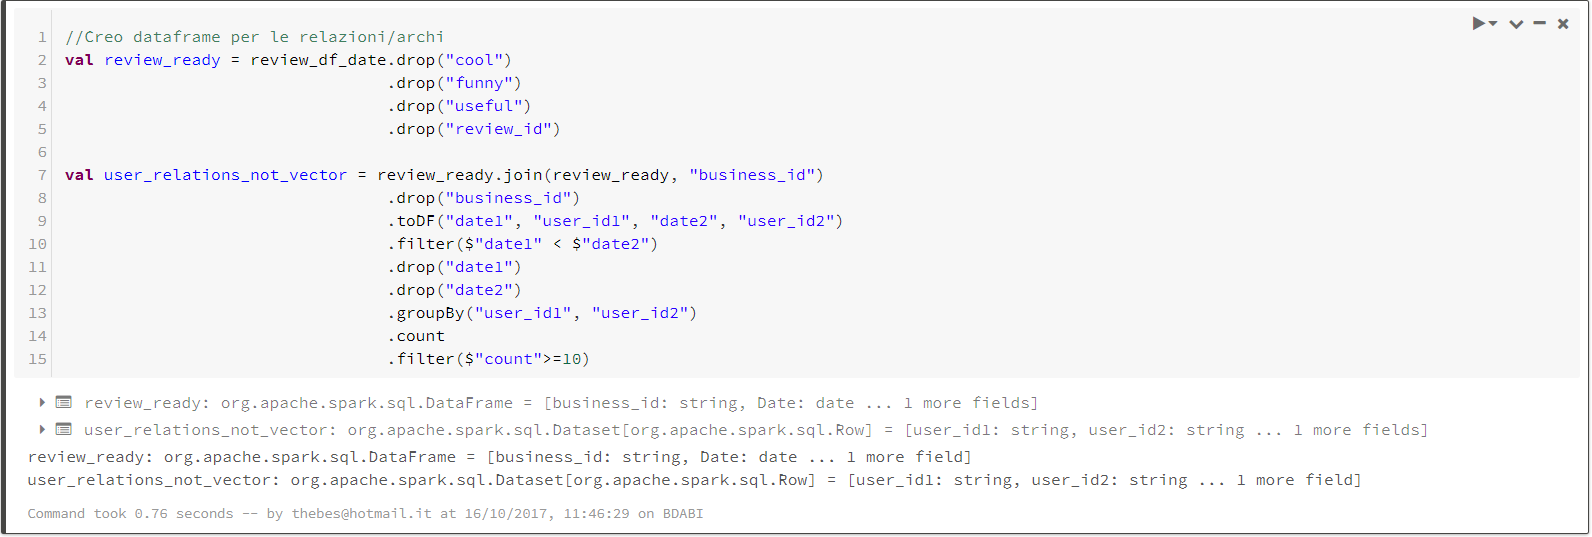
\includegraphics[width=1\linewidth,keepaspectratio]{command_8}
	\caption{Creazione data frame user\_relations\_not\_vector}
	\label{command_8}
\end{figure}

\clearpage

La seguente command prepara i dati al fine di essere elaborati dallo
\textbf{ScalerModel}, fornito dalle librerie di machine learning di Apache Spark.\\
Questo modello permette di applicare la trasformazione \textit{Z-Score} ai dati,
al fine di normalizzarli.\\
Al termine delle operazioni della command, si ha come data frame risultante quello
contenente \textbf{UserId1, UserId2, weight\_zscore}, ovvero le relazioni
che caratterizzeranno il grafo della Social Network.

\begin{figure}[!htbp]
	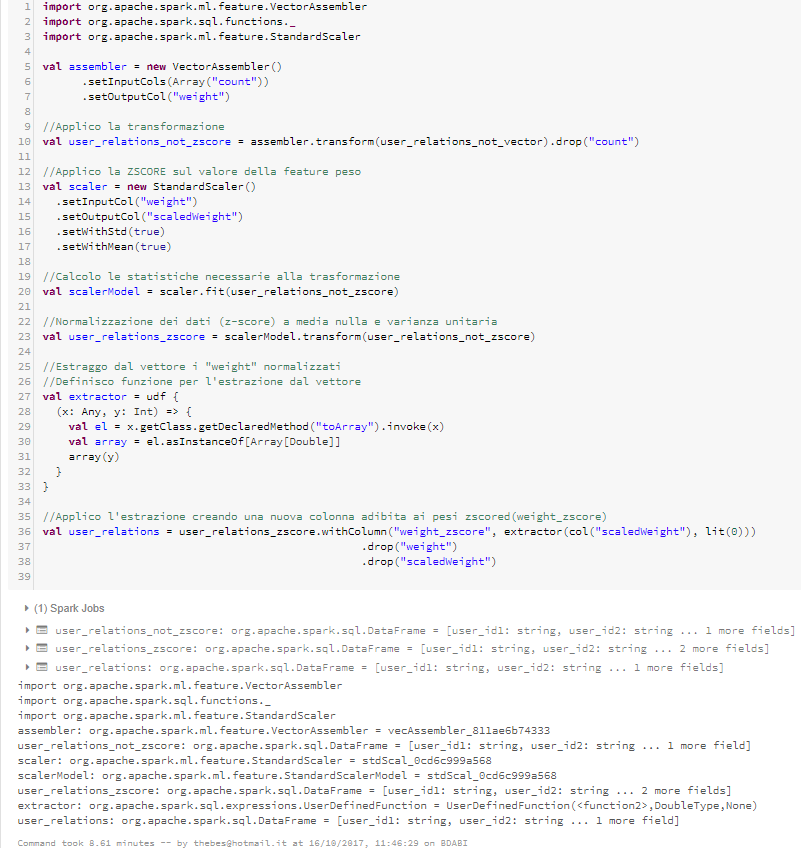
\includegraphics[width=1\linewidth,keepaspectratio]{command_9}
	\caption{Creazione data frame user\_relations finale}
	\label{command_9}
\end{figure}

\clearpage

\section{Creazione data frame dei vertici(users) per il grafo}
La seguente command crea un data frame che, a partire da quello delle relazioni,
prende tutti gli users distinti, così da ottenere i vertici
del grafo.
\begin{figure}[!htbp]
	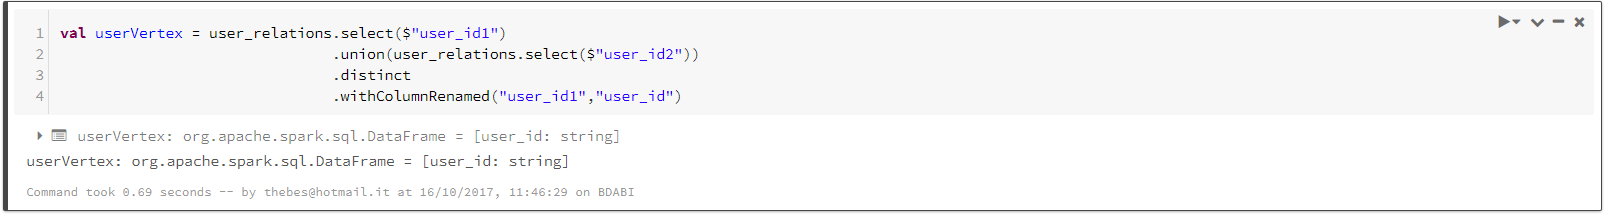
\includegraphics[width=1\linewidth,keepaspectratio]{command_10}
	\caption{Creazione data frame user\_vertex}
	\label{command_10}
\end{figure}

Le due seguenti command preparano il data frame per l'applicazione del modello
\textbf{ScalerModel}, al fine di normalizzare i dati prima di combinarli.\\
In seguito si estraggono le quattro \textit{features normalizzate}(review\_score,
compliment, fans, elite\_score) e se ne calcola una combinazione lineare pesata.
\begin{figure}[!htbp]
	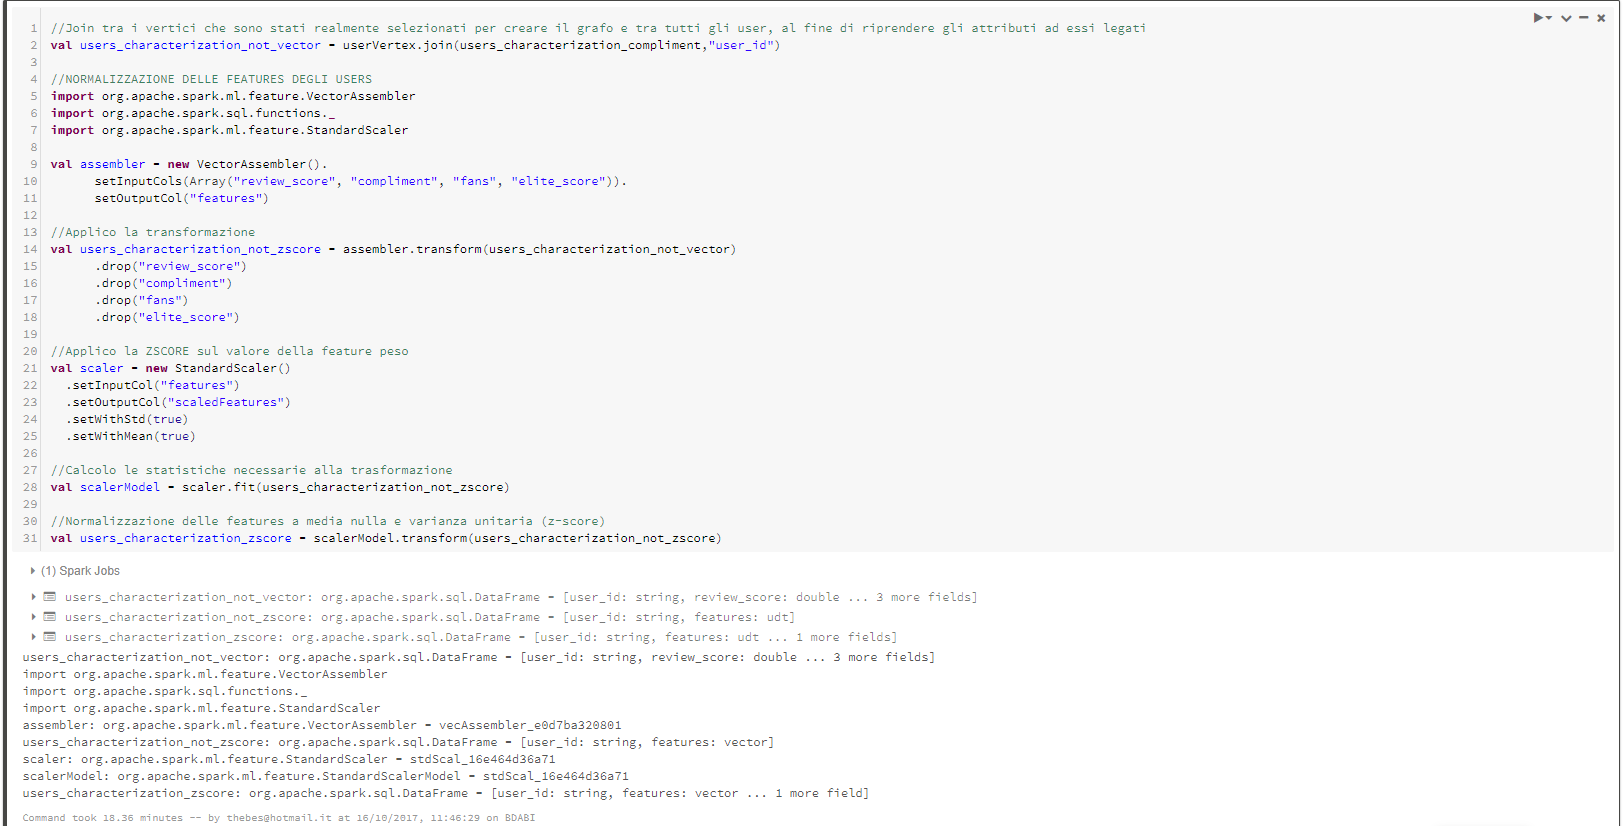
\includegraphics[width=1\linewidth,keepaspectratio]{command_11}
	\caption{Applicazione ScalerModel al data frame user\_vertex}
	\label{command_11}
\end{figure}

\clearpage

Il risultato finale della seguente command è il data frame che associa ad ogni user
lo score ad esso calcolato.\\
Questo score è ottenuto come media pesata delle quattro features scelte per
caratterizzare gli utenti.\\
Inizialmente, i pesi sono stati assegnati con egual valore(0.25).\\
Successivamente saranno mostrati differenti esperimenti al loro variare, al fine
di ottenere una copertura maggiore del grafo.
\begin{figure}[!htbp]
 	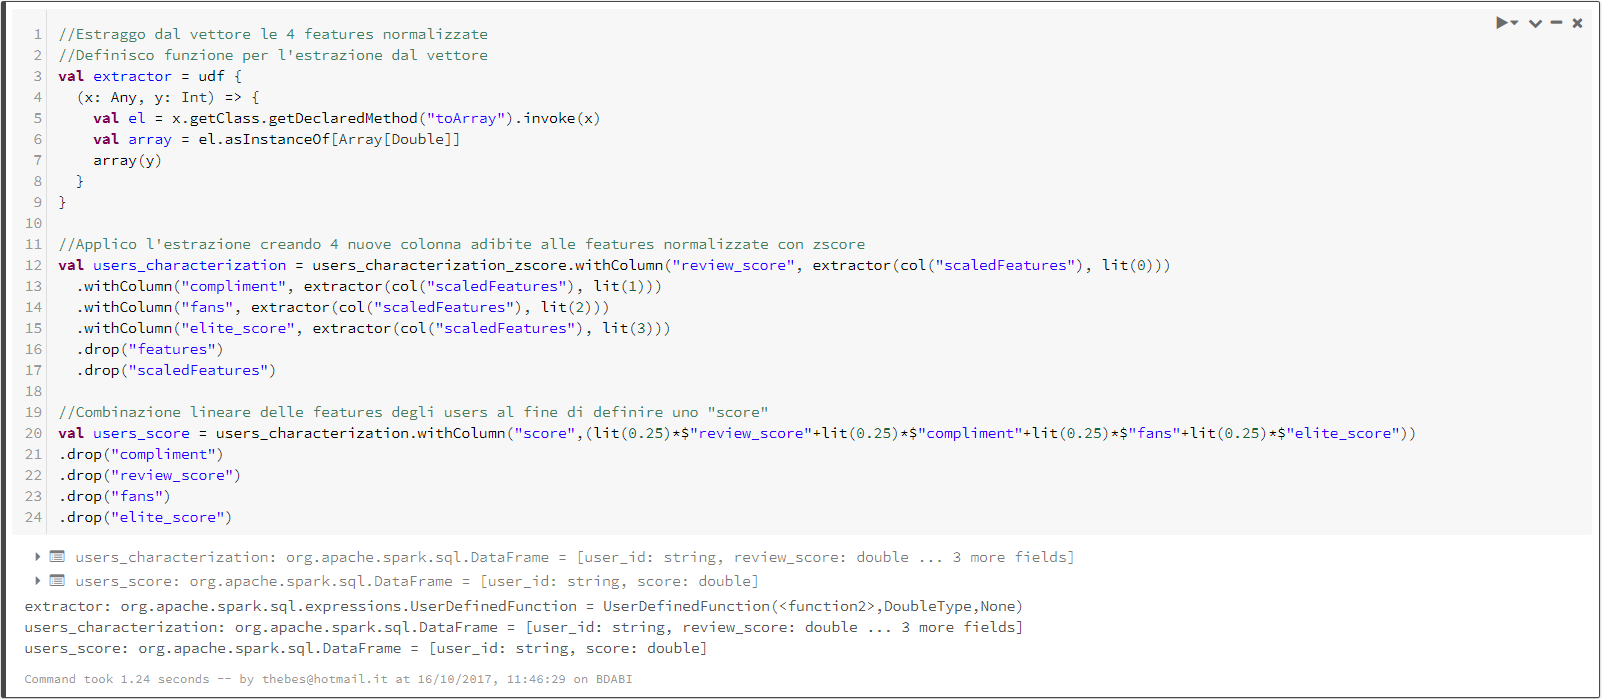
\includegraphics[width=1\linewidth,keepaspectratio]{command_12}
 	\caption{Creazione data frame contenente user e score calcolato}
 	\label{command_12}
\end{figure}
